\documentclass[a4paper,14pt]{extreport}

\usepackage{cmap} % Улучшенный поиск русских слов в полученном pdf-файле
\usepackage[T2A]{fontenc} % Поддержка русских букв
\usepackage[utf8]{inputenc} % Кодировка utf8
\usepackage[english,russian]{babel} % Языки: русский, английский
%\usepackage{pscyr} % Нормальные шрифты

\usepackage{amsmath}

\usepackage{geometry}
\geometry{left=30mm}
\geometry{right=15mm}
\geometry{top=20mm}
\geometry{bottom=20mm}

\usepackage{titlesec}
\titleformat{\section}
	{\normalsize\bfseries}
	{\thesection}
	{1em}{}
\titlespacing*{\chapter}{0pt}{-30pt}{8pt}
\titlespacing*{\section}{\parindent}{*4}{*4}
\titlespacing*{\subsection}{\parindent}{*4}{*4}

\usepackage{setspace}
\onehalfspacing % Полуторный интервал

\frenchspacing
\usepackage{indentfirst} % Красная строка

\usepackage{titlesec}
\titleformat{\chapter}{\LARGE\bfseries}{\thechapter}{20pt}{\LARGE\bfseries}
\titleformat{\section}{\Large\bfseries}{\thesection}{20pt}{\Large\bfseries}

\usepackage{graphicx}
\graphicspath{{inc/img/}}
\DeclareGraphicsExtensions{.png,.jpg}

\usepackage[justification=centering]{caption} % Настройка подписей float объектов

\usepackage[unicode,pdftex]{hyperref} % Ссылки в pdf
\hypersetup{hidelinks}

\usepackage{listings}
\usepackage{xcolor}
\lstdefinestyle{asm}{
	language={[x86masm]Assembler},
	backgroundcolor=\color{white},
	basicstyle=\footnotesize\ttfamily,
	keywordstyle=\color{blue},
	stringstyle=\color{red},
	commentstyle=\color{gray},
	numbers=left,
	numberstyle=\tiny,
	stepnumber=1,
	numbersep=5pt,
	frame=single,
	tabsize=4,
	captionpos=b,
	breaklines=true
}

\lstset{
	literate=
	{а}{{\selectfont\char224}}1
	{б}{{\selectfont\char225}}1
	{в}{{\selectfont\char226}}1
	{г}{{\selectfont\char227}}1
	{д}{{\selectfont\char228}}1
	{е}{{\selectfont\char229}}1
	{ё}{{\"e}}1
	{ж}{{\selectfont\char230}}1
	{з}{{\selectfont\char231}}1
	{и}{{\selectfont\char232}}1
	{й}{{\selectfont\char233}}1
	{к}{{\selectfont\char234}}1
	{л}{{\selectfont\char235}}1
	{м}{{\selectfont\char236}}1
	{н}{{\selectfont\char237}}1
	{о}{{\selectfont\char238}}1
	{п}{{\selectfont\char239}}1
	{р}{{\selectfont\char240}}1
	{с}{{\selectfont\char241}}1
	{т}{{\selectfont\char242}}1
	{у}{{\selectfont\char243}}1
	{ф}{{\selectfont\char244}}1
	{х}{{\selectfont\char245}}1
	{ц}{{\selectfont\char246}}1
	{ч}{{\selectfont\char247}}1
	{ш}{{\selectfont\char248}}1
	{щ}{{\selectfont\char249}}1
	{ъ}{{\selectfont\char250}}1
	{ы}{{\selectfont\char251}}1
	{ь}{{\selectfont\char252}}1
	{э}{{\selectfont\char253}}1
	{ю}{{\selectfont\char254}}1
	{я}{{\selectfont\char255}}1
	{А}{{\selectfont\char192}}1
	{Б}{{\selectfont\char193}}1
	{В}{{\selectfont\char194}}1
	{Г}{{\selectfont\char195}}1
	{Д}{{\selectfont\char196}}1
	{Е}{{\selectfont\char197}}1
	{Ё}{{\"E}}1
	{Ж}{{\selectfont\char198}}1
	{З}{{\selectfont\char199}}1
	{И}{{\selectfont\char200}}1
	{Й}{{\selectfont\char201}}1
	{К}{{\selectfont\char202}}1
	{Л}{{\selectfont\char203}}1
	{М}{{\selectfont\char204}}1
	{Н}{{\selectfont\char205}}1
	{О}{{\selectfont\char206}}1
	{П}{{\selectfont\char207}}1
	{Р}{{\selectfont\char208}}1
	{С}{{\selectfont\char209}}1
	{Т}{{\selectfont\char210}}1
	{У}{{\selectfont\char211}}1
	{Ф}{{\selectfont\char212}}1
	{Х}{{\selectfont\char213}}1
	{Ц}{{\selectfont\char214}}1
	{Ч}{{\selectfont\char215}}1
	{Ш}{{\selectfont\char216}}1
	{Щ}{{\selectfont\char217}}1
	{Ъ}{{\selectfont\char218}}1
	{Ы}{{\selectfont\char219}}1
	{Ь}{{\selectfont\char220}}1
	{Э}{{\selectfont\char221}}1
	{Ю}{{\selectfont\char222}}1
	{Я}{{\selectfont\char223}}1
}


\begin{document}

\begin{titlepage}
	\centering

	{\footnotesize \itshape Государственное образовательное учреждение высшего профессионального образования «Московский Государственный Технический Университет имени Н.~Э.~Баумана»\\}

	\vspace{60mm}

	\textbf{ОТЧЕТ}\\
	По лабораторной работе №1\\
	По курсу: «Операционные системы»\\
	Тема: «Прерывание таймера INT 8h и его функции»\\

	\vspace{60mm}

	\hspace{70mm} Студент:\hfill Керимов~А.~Ш.\\
	\hspace{70mm} Группа: \hfill ИУ7-54Б\\
	%\vspace{5mm}
	\hspace{70mm} Преподаватель:\hfill Рязанова~Н.~Ю.\\

	\vfill
	Москва, 2019
\end{titlepage}


\section*{Листинг обработчика INT 8h}

\begin{lstlisting}[style={asm}]
;; Вызов процедуры sub_1
020A:0746  E8 0070			call	sub_1		; (07B9)

;; Сохранение регистров ES, DS, AX, DX
020A:0749  06				push	es
020A:074A  1E				push	ds
020A:074B  50				push	ax
020A:074C  52				push	dx

;; Установка сегмента данных
020A:074D  B8 0040			mov	ax,40h
020A:0750  8E D8			mov	ds,ax
020A:0752  33 C0			xor	ax,ax			; Zero register
020A:0754  8E C0			mov	es,ax

;; Инкремент счётчика реального времени по известному адресу в области данных BIOS
;  Инкремент двух младших байтов счётчика реального времени по адресу 0040:006C
020A:0756  FF 06 006C		inc	word ptr ds:[6Ch]	; (0040:006C=0E873h)
020A:075A  75 04			jnz	loc_1				; Jump if not zero
;  Инкремент двух старших байтов счётчика реально времени по адресу 0040:006E
020A:075C  FF 06 006E		inc	word ptr ds:[6Eh]	; (0040:006E=0Ch)

;; Сброс счётчика реального времени при наступлении новых суток
020A:0760			loc_1:
020A:0760  83 3E 006E 18	cmp	word ptr ds:[6Eh],18h ; (0040:006E=0Ch)
020A:0765  75 15			jne	loc_2				  ; Jump if not equal
020A:0767  81 3E 006C 00B0	cmp	word ptr ds:[6Ch],0B0h; (0040:006C=0E873h)
020A:076D  75 0D			jne	loc_2				  ; Jump if not equal
;  Обнуление двух старших байтов счётчика реального времени по адресу 0040:006E
020A:076F  A3 006E			mov	word ptr ds:[6Eh],ax  ; (0040:006E=0Ch)
;  Обнуление двух младших байтов счётчика реального времени по адресу 0040:006C
020A:0772  A3 006C			mov	word ptr ds:[6Ch],ax  ; (0040:006C=0E873h)
;  Установка флага прошедших суток по адресу 0040:0070
020A:0775  C6 06 0070 01	mov	byte ptr ds:[70h],1	  ; (0040:0070=0)
020A:077A  0C 08			or	al,8

;; Декремент счётчика времени до отключения моторчика дисковода по известному адресу в области данных BIOS
020A:077C			loc_2:
020A:077C  50				push	ax
020A:077D  FE 0E 0040		dec	byte ptr ds:[40h]		; (0040:0040=2Bh)
020A:0781  75 0B			jnz	loc_3					; Jump if not zero
;  Установка флага отключения моторчика дисковода
020A:0783  80 26 003F F0	and	byte ptr ds:[3Fh],0F0h	; (0040:003F=0)
;  Посылание команды отключения OCh в порт дисковода 3F2h
020A:0788  B0 0C			mov	al,0Ch
020A:078A  BA 03F2			mov	dx,3F2h
020A:078D  EE				out	dx,al	; port 3F2h, dsk0 contrl output

;; Вызов прерывания 1Ch
020A:078E			loc_3:
020A:078E  58				pop	ax
;  Установлен ли флаг разрешения прерываний IF?
020A:078F  F7 06 0314 0004	test	word ptr ds:[314h],4	; (0040:0314=3200h)
020A:0795  75 0C			jnz	loc_4			; Jump if not zero
;  Косвенный вызов прерывания 1Ch
020A:0797  9F				lahf				; Load ah from flags
020A:0798  86 E0			xchg	ah,al
020A:079A  50				push	ax
020A:079B  26: FF 1E 0070	call	dword ptr es:[70h]	; (0000:0070=6ADh)
020A:07A0  EB 03			jmp	short loc_5				; (07A5)
020A:07A2  90				nop
;  Вызов прерывания 1Сh
020A:07A3			loc_4:
020A:07A3  CD 1C			int	1Ch		; Timer break (call each 18.2ms)

;; Вызов процедуры sub_1
020A:07A5			loc_5:
020A:07A5  E8 0011			call	sub_1	; (07B9)

;; Сброс контроллера прерываний записью 20h в порт 20h
020A:07A8  B0 20			mov	al,20h		; ' '
020A:07AA  E6 20			out	20h,al		; port 20h, 8259-1 int command
;  al = 20h, end of interrupt

;; Восстановление регистров DX, AX, DS, ES
020A:07AC  5A				pop	dx
020A:07AD  58				pop	ax
020A:07AE  1F				pop	ds
020A:07AF  07				pop	es

;; Завершение обработчика прерывания 8h
020A:07B0  E9 FE99			jmp	$-164h		; (07B0-164=064C)

020A:064C  1E				push	ds
020A:064D  50				push	ax
; ...
020A:06AA  58				pop	ax
020A:06AB  1F				pop	ds
020A:06AC  CF				iret			; Interrupt return
\end{lstlisting}

\section*{Листинг процедуры sub\_1}

\begin{lstlisting}[style={asm}]
					sub_1		proc	near

;; Сохранение регистров DS, AX
020A:07B9  1E					push	ds
020A:07BA  50					push	ax

;; Установка сегмента данных = 0040
020A:07BB  B8 0040				mov	ax,40h
020A:07BE  8E D8				mov	ds,ax

; Загрузка EFLAGS в AH
020A:07C0  9F					lahf				 ; Load ah from flags
020A:07C1  F7 06 0314 2400		test	word ptr ds:[314h],2400h		; (0040:0314=3200h)
020A:07C7  75 0C				jnz	loc_7			 ; Jump if not zero
020A:07C9  F0> 81 26 0314 FDFF	lock	and	word ptr ds:[314h],0FDFFh	; (0040:0314=3200h)
020A:07D0			loc_6:
020A:07D0  9E					sahf				; Store ah into flags
020A:07D1  58					pop	ax
020A:07D2  1F					pop	ds
020A:07D3  EB 03				jmp	short loc_8		; (07D8)
020A:07D5			loc_7:
020A:07D5  FA					cli					; Disable interrupts
020A:07D6  EB F8				jmp	short loc_6		; (07D0)
020A:07D8			loc_8:
020A:07D8  C3					retn
sub_1		endp
\end{lstlisting}

\pagebreak

\section*{Схема алгоритма обработчика INT 8h}

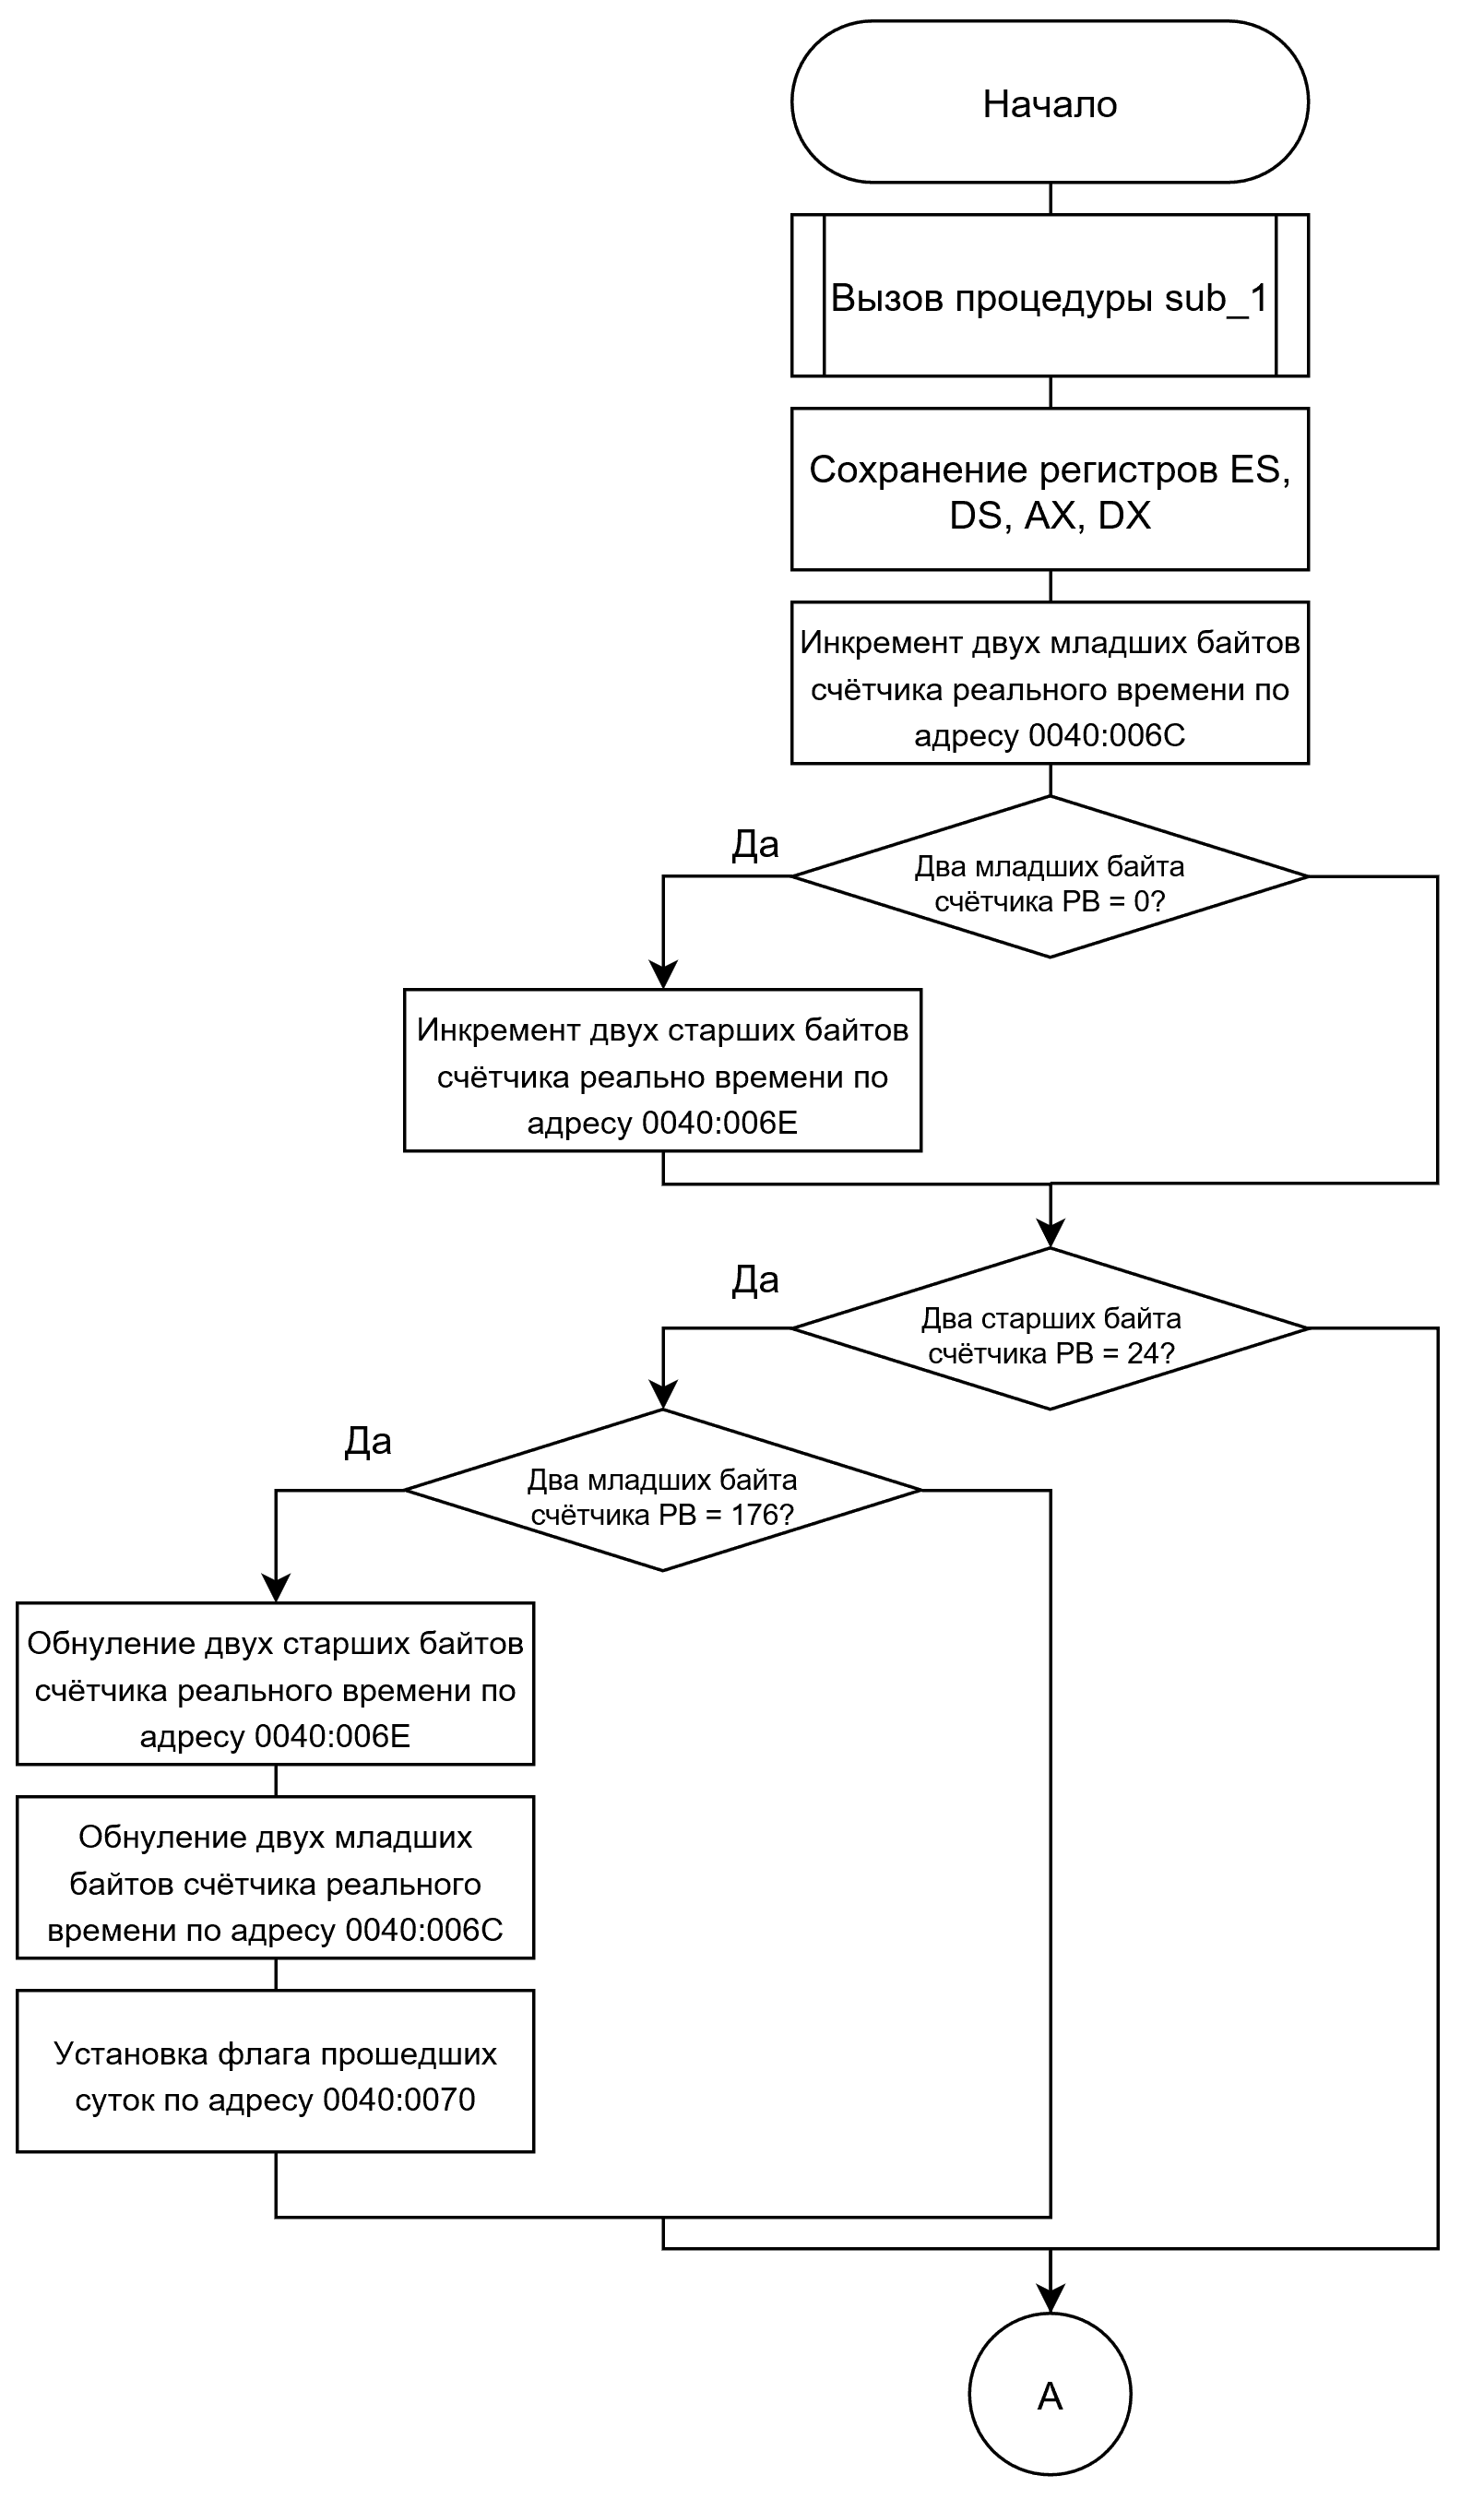
\includegraphics[height=240mm]{int8h_1}

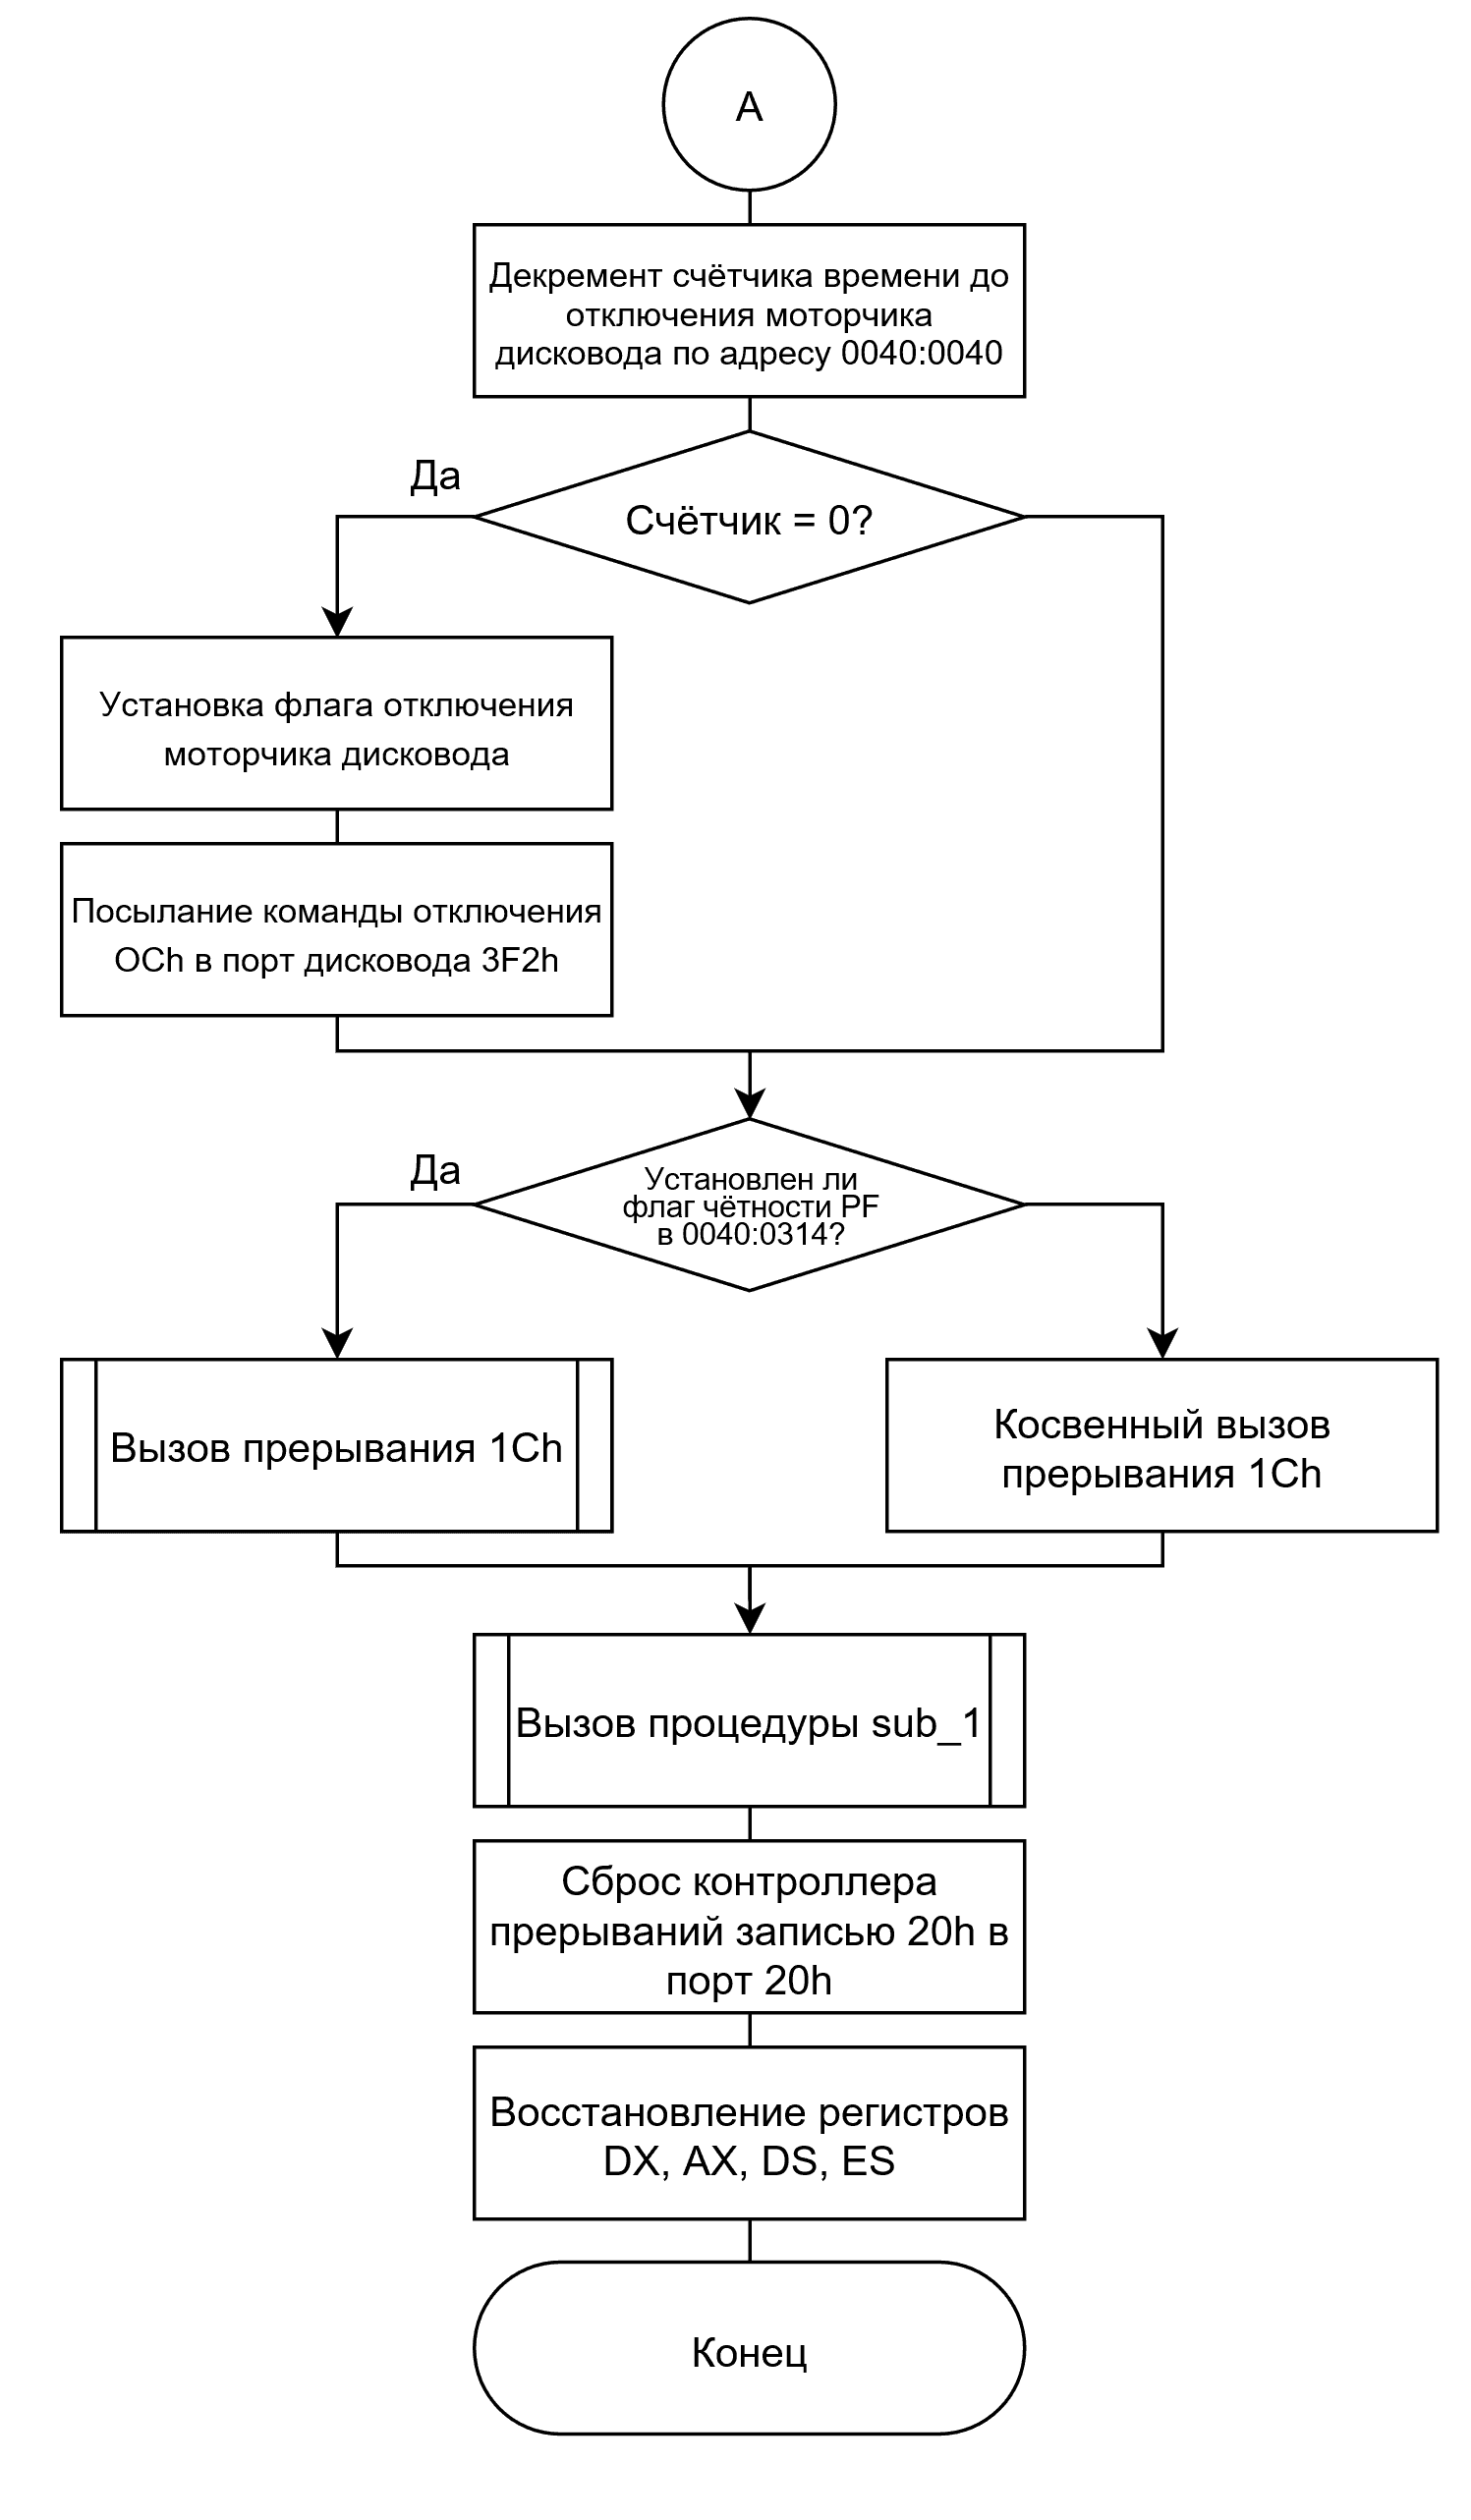
\includegraphics[height=260mm]{int8h_2}

\section*{Схема алгоритма процедуры sub\_1}

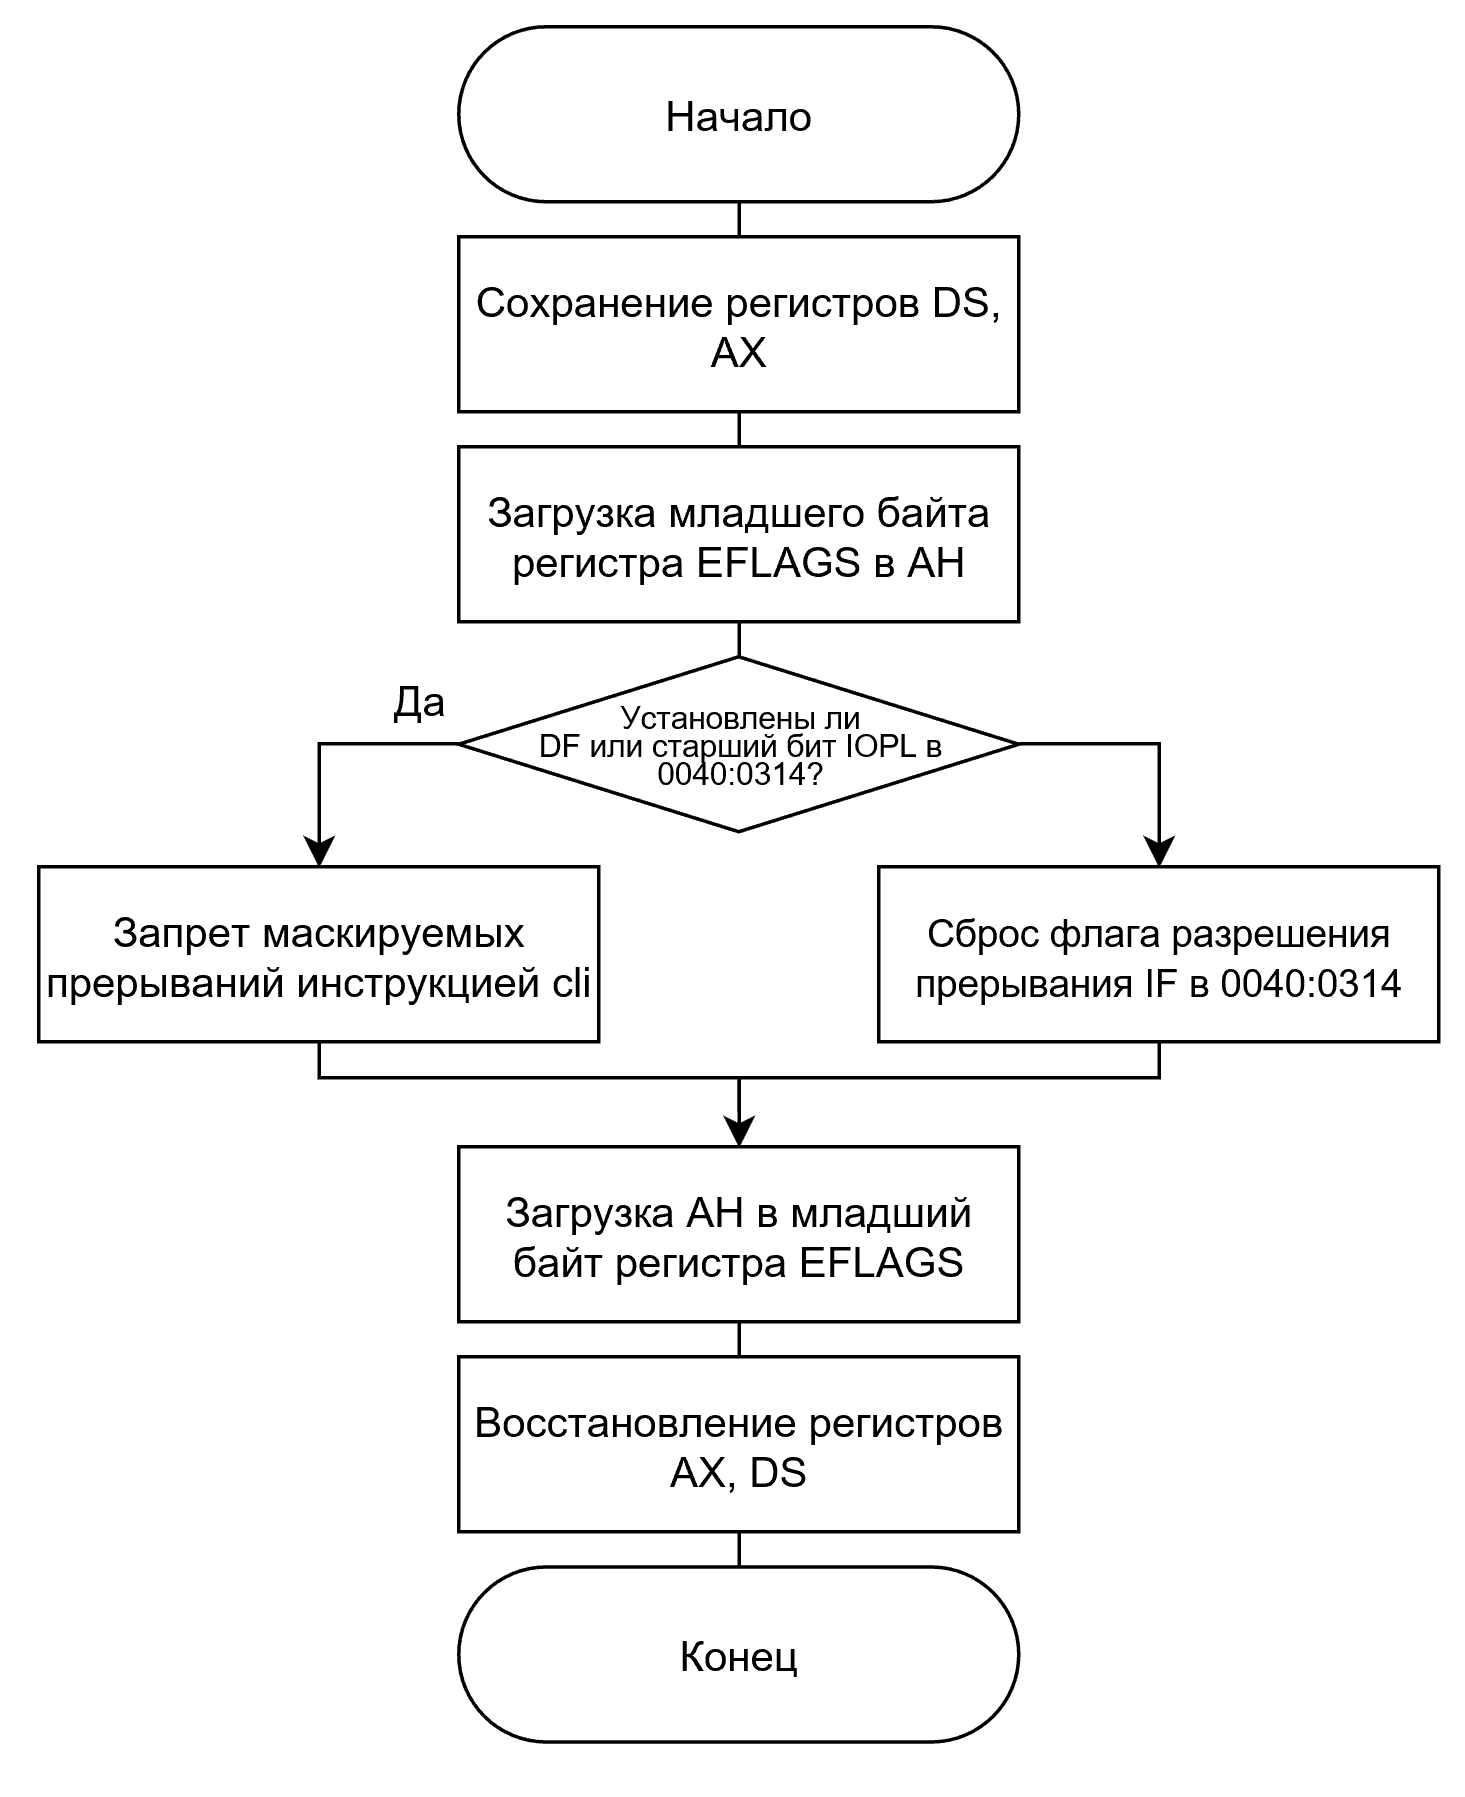
\includegraphics[height=180mm]{int8h_3}

\end{document}
